% \documentclass{book}

\documentclass[12pt]{article}
\usepackage[pdfborder={0 0 0.5 [3 2]}]{hyperref}%
\usepackage[left=1in,right=1in,top=1in,bottom=1in]{geometry}%
\usepackage[shortalphabetic]{amsrefs}%
\usepackage{amsmath}
\usepackage{enumerate}
\usepackage{enumitem}
\usepackage{amssymb}                
\usepackage{amsmath}                
\usepackage{amsfonts}
\usepackage{amsthm}
\usepackage{bbm}
\usepackage[table,xcdraw]{xcolor}
\usepackage{tikz}
\usepackage{float}
\usepackage{booktabs}
\usepackage{svg}
\usepackage{mathtools}
\usepackage{cool}
\usepackage{url}
\usepackage{graphicx,epsfig}
\usepackage{makecell}
\usepackage{array}

\graphicspath{ {images/} }

\begin{document}

\title{}
\author{\vspace{-10ex} }

\begin{center}
{\LARGE APMA 1650 -- Homework 1}\\
\vspace{5mm}
{\large Due Tuesday, July 5, 2016}\\
\vspace{5mm}
Homework is due during class or by 3:45 pm in the homework drop box in 182 George St.\\
Show all of your work used in deriving your solutions.
\end{center}

\begin{enumerate}
\item Suppose you flip a fair coin 50 times. Answer the following questions. You may leave the answers in terms of binomial coefficients and exponents, i.e. you don't have to expand out all the things.
\begin{enumerate}
\item What is the size of the sample space for this experiment, i.e. how many outcomes are possible?\\

Since there are two possible outcomes for each coin flip (H or T), and there are 50 flips, by the Basic Principle of Counting the sample space contains $2^{50}$ possible outcomes.

\item What is the probability that you flip exactly 10 heads?\\

An outcome can be represented as a string of 50 Hs and Ts. Exactly 10 heads means a string composed of 10 Hs and 40 Ts. Since there are $\binom{50}{10}$ such strings, the probability is:
\[
\frac{\binom{50}{10}}{2^{50}}
\]

\item What is the probability that you flip at least 10 heads?
At least 10 heads means not flipping $0, 1, 2, \dots, 9$ heads. Thus we have the probability of at least 10 heads in a row is:
\[
1 - \frac{\binom{50}{0}}{2^{50}} - \frac{\binom{50}{1}}{2^{50}} - \cdots - \frac{\binom{50}{9}}{2^{50}}
\]
You could also sum up the probabilties of $10, 11, 12, \dots, 50$ heads.

\item What is the probability that you never flip two heads in a row or two tails in a row?
The only way to do this is to alternate heads and tails, i.e. to flip HTHT...HT or THTH...TH. Thus there are only two ways to do this, so the probability is:
\[
\frac{2}{2^{50}} = \frac{1}{2^{49}}
\] 
\end{enumerate}

\item You are performing an experiment in which you survey $n$ randomly-selected people and record their birthday. Assume that there are only 365 possible birthdays, i.e. ignore leap year. Also assume that the probability of having any birthday is equally likely. You may leave the first two parts in terms of binomial coefficients and exponents, but I want a specific number for $n$ in the third part.
\begin{enumerate}
\item What is the size of the sample space for this experiment, i.e. how many outcomes are possible?\\

Each of $n$ people has 365 birthdays to choose from, so the size of the sample space is $365^n$.

\item Take $n = 5$. What is the probability that each of the 5 people has a different birthday?\\

In order to not duplicate, the first person has 365 days to choose from, the second 364 to choose from, etc. Since the sample space has size $365^5$, the probability of no duplicate birthdays is:
\[
\frac{ 365 \cdot 364 \cdot 363 \cdot 362 \cdot 361}{365^5}
\]

\item What is the smallest value of $n$ such that the probability is at least 0.5 that at least two people share a birthday? (This may take a little guesswork with a calculator, but I promise it is not too bad.)\\

We want the value of $n$ such that the probability that two or more people share a birthday is $\geq$ 0.5. This is the same as the value of $n$ such that the probabilty that no two people share a birthday is $\leq$ 0.5. In other words, generalizing part b, we want the smallest $n$ such that:
\[
\frac{ 365 \cdot 364 \cdot 363 \dots \cdot (365 - n + 1)}{365^n} \leq 0.5
\] 
For $n = 22$, this is 0.524. For $n = 23$, this is 0.492. Thus the smallest $n$ for which this holds is 23.

\end{enumerate}

\item You enlist a friend from materials science to construct a very special unfair six-sided die. The die looks like a standard die, i.e. it it cubical and has the numbers 1, 2, 3, 4, 5, and 6 on its faces. On this die, the probability of rolling any number is directly proportional to that number. For example, you are twice as likely to roll a 6 as a 3. 
\begin{enumerate}
\item What is the probability of rolling each of the six numbers?\\
Let $p$ be the the probabiltiy of rolling a 1. Then the probability of rolling a 2 is $2p$, 3 is $3p$, etc. In other words, the probability of rolling $k$ is $kp$, $k = 1, 2, 3, 4, 5, 6$. Since the probabilities must sum to 1:
\[
1 = p + 2p + 3p + 4p + 5p + 6p = 21p
\]
Thus $p = 1/7$. We then have probabilties:
\begin{figure}[H]
\centering
\begin{tabular}{l@{\hskip 2cm}l}
\toprule
Die roll & probability\\
\midrule
1 & 1/21\\
2 & 2/21\\
3 & 3/21\\
4 & 4/21\\
5 & 5/21\\
6 & 6/21\\
\bottomrule
\end{tabular}
\end{figure}

\item What is the probabiltiy of rolling an odd number?\\
Adding up the probabilities for 1, 3, and 5, we get 9/21.

\end{enumerate}

\item Consider the grid of points shown below. You start at (0, 0) and take one step either up or to the right with each move. You keep moving until you reach (10, 10). You can never leave the grid. For example, if you reach the point (4, 10), you can only move to the right from that point onwards. Assume that each possible path is equally likely. Answer the following questions. You may leave the answers in terms of binomial coefficients and exponents.
\begin{enumerate}
\item What is the size of the sample space, i.e. how many possible paths are there from (0, 0) to (10, 10)?\\

To get from (0, 0) to (10, 10) we must take 10 steps right and 10 steps up. These may be done in any order. If we think of a path as string of 20 Us or Rs, where we have exaclty 10 Us and 10 Rs, the number of such strings (thus the number of possible paths) is $\binom{20}{10}$.

\item What is the probability that a path passes through (5, 5)?\\

A path that goes through (5,5) must go from (0, 0) to (5, 5) then from (5, 5) to (10, 10). Using the logic above, there are $\binom{10}{5}$ paths from (0, 0) to (5, 5) and $\binom{10}{5}$ paths from (5, 5) to (10, 10). Multiplying these together, there are $\binom{10}{5}^2$ paths from (0, 0) to (10, 10) which pass through (5, 5). Thus the probability of this occurring is:
\[
\frac{\binom{10}{5}^2 }{ \binom{20}{10}}
\]
\end{enumerate}
\begin{figure}[H]
\centering
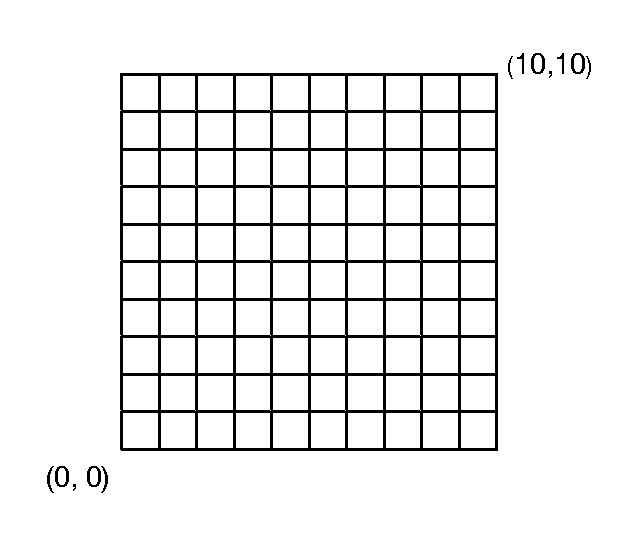
\includegraphics[width=10cm]{grid.eps}
\end{figure}

\item Powerball is an American lottery game offered by 44 states (including Rhode Island). To play the game, you select 5 distinct numbers from a set of 69 white balls (numbered 1 - 69) and one number from a set of 26 red Powerballs (numbered 1 - 26). In each drawing, five white balls and one red Powerball are selected\footnote{If you Google ``Powerball'', today's numbers are displayed at the top of the search results. In asking this question, the instructor is not condoning playing Powerball. }. The order of the white balls does not matter. (In the official Powerball drawing, the white balls are listed in ascending order.) 
\begin{enumerate}
\item You win the jackpot if you match all 5 white balls and the Powerball. What is the probability that you win the jackpot?\\

First note that there are $\binom{69}{5}$ possible draws for the 5 white balls (since order does not matter). To win the jackpot, you need to get 1 out of these $\binom{69}{5}$ possible draws for the 5 white balls and 1 out of the 26 possible draws for the powerball. The probability is:
\[
\frac{1}{\binom{69}{5}}\frac{1}{26}, \text{  approximately 1 in 292,201,338}
\]

\item If you match all 5 white balls but do not match the Powerball, you win \$1,000,000. What is the probability that this occurs?\\

This is the same as the above except we don't want to match the Powerball. Since there are 25/26 ways to not match the Powerball, this is:
\[
\frac{1}{\binom{69}{5}}\frac{25}{26}, \text{  approximately 1 in 11,688,054}
\]

\item If you match the Powerball but do not match \emph{any} of the white balls, you win \$4. What is the probability that this occurs?\\

To not match any of the white balls, your 5 balls must all be chosen from the 64 balls which are not winners. There are $\binom{64}{5}$ ways to choose 5 balls from the 64 non-winning balls. Since there is a 1/26 probability of matching the Powerball, the probability of this event is:
\[
\frac{ \binom{64}{5} }{\binom{69}{5}}\frac{1}{26}, \text{  approximately 1 in 38}
\]

\item If you match \emph{exactly} 3 white balls (so you don't match the other two balls) and the Powerball, you win \$100. What is the probability that this occurs?\\

To match exactly 3 white balls, you choose 3 balls from the 5 winning balls ($\binom{5}{3}$ ways to do this) and you choose 2 bals from the 64 non-winning balls ($\binom{64}{2}$ ways to do this). Since there is a 1/26 probability of matching the Powerball, the probability of this event is:
\[
\frac{ \binom{5}{3} \binom{64}{2} }{\binom{69}{5}}\frac{1}{26}, \text{  approximately 1 in 14,494}
\]

\end{enumerate}

\end{enumerate}
\end{document}

